\documentclass[a4paper]{extarticle}
\usepackage[utf8]{inputenc}
\usepackage[a4paper, margin=1in]{geometry}

\usepackage{amssymb}
\usepackage{amsmath}
\usepackage{enumitem}
\usepackage{tcolorbox}
\usepackage{fancyhdr}
\usepackage{graphicx}
\usepackage{float}

\setlength{\parindent}{0em}
\setlength{\parskip}{0.4em}

\definecolor{theoremblue}{RGB}{1, 73, 124}
\definecolor{corollaryblue}{RGB}{70, 143, 175}
\definecolor{exampleblue}{RGB}{137, 194, 217}

\newtcolorbox{tbox}{colback=theoremblue!20,colframe=theoremblue,
boxrule=0pt,arc=0pt,boxsep=2pt,left=2pt,right=2pt,leftrule=2pt}

\newtcolorbox{cbox}{colback=corollaryblue!20,colframe=corollaryblue,
boxrule=0pt,arc=0pt,boxsep=2pt,left=2pt,right=2pt,leftrule=2pt}

\newtcolorbox{ebox}{colback=exampleblue!20,colframe=exampleblue,
boxrule=0pt,arc=0pt,boxsep=2pt,left=2pt,right=2pt,leftrule=2pt}

\title{FMFP - Lecture Notes Week 2}
\author{Ruben Schenk, ruben.schenk@inf.ethz.ch}
\date{\today}

\pagestyle{fancy}
\fancyhf{}
\rhead{ruben.schenk@inf.ethz.ch}
\rfoot{Page \thepage}
\lhead{FMFP - Lecture Notes Week 2}

\begin{document}

\maketitle
\newpage

\subsection{First-Order Logic}

\subsubsection{Syntax}

In \textbf{first-order logic} we have two syntactic categories: \textbf{terms} and \textbf{formulae.}

A \textbf{signature} consists of a set of function symbols \(\mathcal{F}\) and a set of predicate symbols \(\mathcal{P}\).
We write \(f^k\) (or \(p^k\)) to indicate function symbol \(f\) (or predicate symbol \(p\)) has arity \(k \in \mathcal{N}\). Constants are \(0\)-ary function symbols.

Now, let \(\mathcal{V}\) be a set of variables. Then:

\begin{tbox}
    \textbf{Definition:} \(Term\), the \textbf{terms of first-order logic,} is the smallest set where:
    \begin{enumerate}
        \item \(x \in Term\) if \(x \in V\), and
        \item \(f^n(t_1,..., \, t_n) \in Term\) if \(f^n \in \mathcal{F}\) and \(t_i \in Term\), for all \(1 \leq i \leq n\).
    \end{enumerate}
\end{tbox}

\begin{tbox}
    \textbf{Definition:} \(Form\), the \textbf{formulae of first-order logic,} is the smallest set where:
    \begin{enumerate}
        \item \(\bot \in Form\),
        \item \(p^n(t_1,..., \, t_n) \in Form\) if \(p^n \in \mathcal{P}\) and \(t_j \in Term\), for all \(1 \leq j \leq n\),
        \item \(A \circ B \in Form\) if \(A \in Form\), \(B \in Form\), and \(\circ \in \{\land, \, \lor, \, \to\}\), and
        \item \(Qx.A \in Form\) if \(A \in Form\), \(x \in \mathcal{V}\), and \(Q \in \{\forall, \, \exists\}\).
    \end{enumerate}
\end{tbox}

Each occurrence of each variable in a formula is either \textbf{bound} or \textbf{free.} A variable occurrence \(x\) in a formula \(A\) is \textbf{bound} if \(x\) occurs within a subformula \(B\) of \(A\) of the form \(\exists x.B\) or \(\forall x.B\).

\subsubsection{Binding and \(\alpha\)-conversion}

Names of bound variables are irrelevant, they just encode the binding structure. We can rename \textit{bound} variables, this process is called \textbf{\(\alpha\)-conversion}.

It is important to note that the renaming must \textit{preserve the binding structure!}

Some notes on bindings and parentheses:

\begin{itemize}
    \item \(\land\) binds stronger than \(\lor\), and \(\lor\) binds stronger than \(\to\).
    \item \(\to\) associates to the right, \(land\) and \(lor\) to the left.
    \item Negation binds stronger than binary operators.
    \item Quantifiers extend to the right as far as possible: to the end of the line or ')'
\end{itemize}

\begin{figure}[H]
    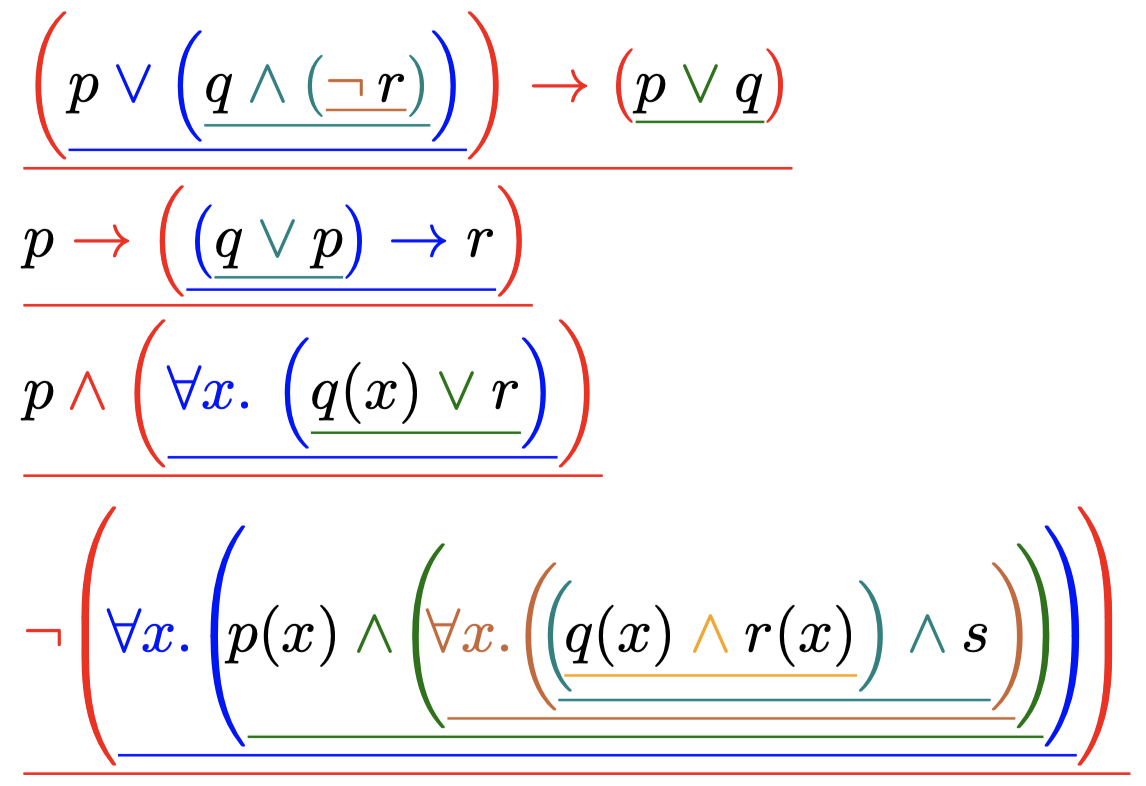
\includegraphics[width=7cm]{../images/FMFP_Fig2-1}
    \centering
\end{figure}

\subsubsection{Semantics}

A \textbf{structure} is a pair \(\mathcal{S} = \langle U_{\mathcal{S}}, \, I_{\mathcal{S}} \rangle\) where \(U_{\mathcal{S}}\) is a nonempty set, the \textbf{universe,} and \(I_{\mathcal{S}}\) is a mapping where:

\begin{enumerate}
    \item \(I_{\mathcal{S}}(p^n)\) is an \(n\)-ary relation on \(U_{\mathcal{S}}\), for \(p^n \mathcal{P}\), and
    \item \(I_{\mathcal{S}}(f^n)\) is an \(n\)-ary (total) function on \(U_{\mathcal{S}}\), for \(f^n \in \mathcal{F}\)
\end{enumerate}

As a shorthand, we write \(p^{\mathcal{S}}\) for \(I_{\mathcal{S}}(p)\) and \(f^{\mathcal{S}}\) for \(I_{S}(f)\).

An \textbf{interpretation} is a pair \(\mathcal{I} = \langle \mathcal{S}, \, v \rangle\), where \(\mathcal{S} = \langle U_{\mathcal{S}}, \, I_{\mathcal{S}}\) is a structure and \(v : \mathcal{V} \to U_{\mathcal{S}}\) is a valuation.

The \textbf{value} of a term \(t\) under the interpretation \(\mathcal{I} = \langle S, \, v \rangle\) is written as \(\mathcal{I}(t)\) and defined by:

\begin{enumerate}
    \item \(\mathcal{I}(x) = v(x)\), for \(x \in \mathcal{V}\), and
    \item \(\mathcal{I}(f(t_1,..., \, t_n)) = f^{\mathcal{S}}(\mathcal{I}(t_1),..., \, \mathcal{I}(t_n))\).
\end{enumerate}

\textbf{Satisfiability} is the smallest relation \(\vDash \subseteq Interpretations \times Form\) satisfying:

\begin{itemize}
    \item \(\langle \mathcal{S}, \, v \rangle \vDash p(t_1,..., \, t_n)\) if \((\mathcal{I}(t_1),..., \, \mathcal{I}(t_n)) \in p^{\mathcal{S}}\), where \(\mathcal{I} = \langle \mathcal{S}, \, v\).
    \item \(\langle \mathcal{S}, \, v \rangle \vDash \forall x.A\) if \(\langle \mathcal{S}, \, v[x \to a] \rangle \vDash A\), for all \(a \in U_{\mathcal{S}}\).
    \item \(\langle \mathcal{S}, \, v \rangle \vDash \exists x.A\) if \(\langle \mathcal{S}, \, v[x \to a] \rangle \vDash A\), for some \(a \in U_{\mathcal{S}}\).
\end{itemize}

Here, \(v[x \to a]\) is the valuation \(v'\) identical to \(v\), except that \(v'(x) = a\).

When \(\langle \mathcal{S}, \, v \rangle \vDash A\), we say that \(A\) \textit{is satisfied with respect to} \(\langle \mathcal{S}, \, v \rangle\) or \(langle \mathcal{S}, \, v \rangle\) is a \textbf{model} of \(A\). Note that if \(A\) does not have free variables, satisfaction does not depend on the valuation \(v\). We write \(\mathcal{S} \vDash A\). When every interpretation is a model, we write \(\vDash A\) and say that \(A\) is \textbf{valid.}

\(A\) is \textbf{satisfiable} if there is at least one model for \(A\) (and said to be \textbf{contradictory} otherwise).

\begin{ebox}
    \textbf{Example:} Consider the following examples:

    \begin{itemize}
        \item \(\forall x. \exists y. y*2 = x\) satisfied w.r.t. rationals.
        \item \(\forall x. \forall y. x < y \to \exists z.x < z \land z < y\) satisfied w.r.t. any dense order.
        \item \(\exists x . x \neq 0\) satisfied w.r.t. structures \(\mathcal{S}\) with \(\geq 2\) elements in \(U_{\mathcal{S}}\).
        \item \((\forall x . p(x, \, x)) \to p(a, \, a)\) is valid.
    \end{itemize}
\end{ebox}

\subsubsection{Substitution}

\textbf{Substitution} describes the process of replacing in \(A\) all occurrences of a free variable \(x\) with some term \(t\). We write \(A[x \to t]\) to indicate the substitution.

\begin{ebox}
    \textbf{Example:}
    \begin{align*}
        A &\equiv \exists y . y * x = x * z \\
        A[x \to 2 - 1] &\equiv \exists y . y * (2 - 1) = (2 - 1) * z \\
        A[x \to z] &\equiv \exists y . y * z = z * z
    \end{align*}
\end{ebox}

All free variables of \(t\) must still be free in \(A[x \to t]\). Avoid \textit{capture!} If necessary, \(\alpha\)-convert \(A\) before substitution.

\subsubsection{Universal Quantification}

The rules are as follows:

\begin{figure}[H]
    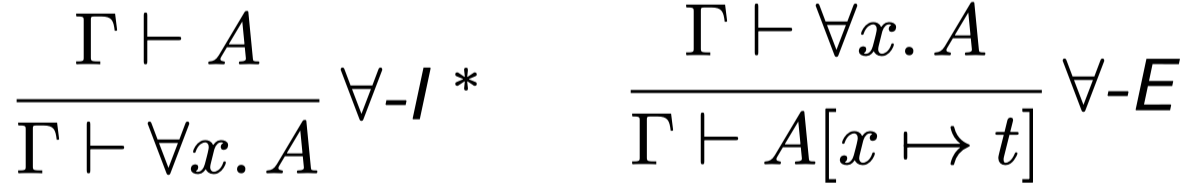
\includegraphics[width=7cm]{../images/FMFP_Fig2-2}
    \centering
\end{figure}

The side condition \(*\) is: \(x\) must not be free in any assumption in \(\Gamma\).

\subsubsection{Existential Quantification}

The rules are as follows:

\begin{figure}[H]
    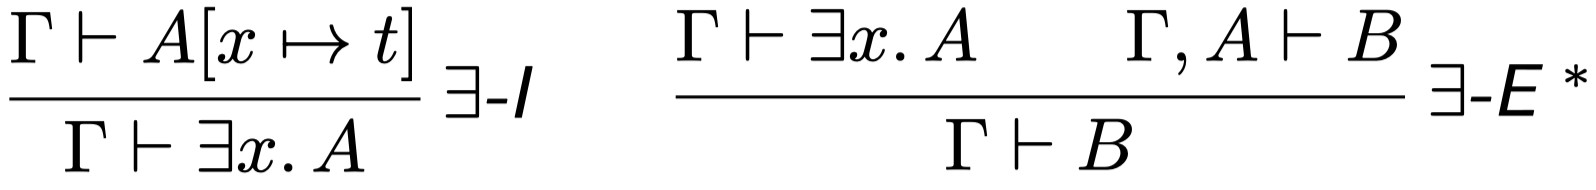
\includegraphics[width=9cm]{../images/FMFP_Fig2-3}
    \centering
\end{figure}

The side condition \(*\) is: \(x\) is neither free in \(B\) nor free in \(\Gamma\).

\subsection{Equality}

\textbf{Equality} is a logical symbol with associated proof rules. One speaks of \textit{first-order logic with equality} rather than equality just being another predicate:

\begin{itemize}
    \item Extended language: \(t_1 = t_2 \in Form\) if \(t_1, t_2 \in Term\)
    \item extended definition of semantic entailment \(\vDash\): \(\mathcal{I} \vDash t_1 = t_2\) if \(\mathcal{I}(t_1) = \mathcal{I}(t_2)\)
\end{itemize}

Equality is an \textit{equivalence} relation with the following rules:

\begin{figure}[H]
    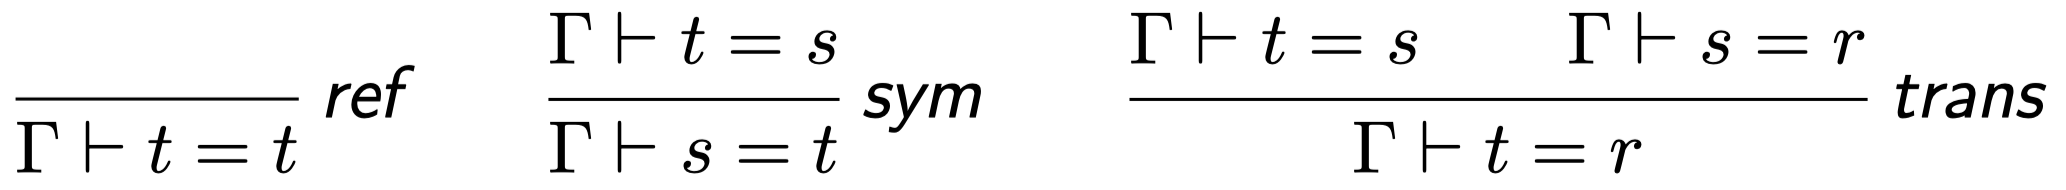
\includegraphics[width=12cm]{../images/FMFP_Fig2-4}
    \centering
\end{figure}

And equality is also a \textit{congruence} on terms and all definable relations:

\begin{figure}[H]
    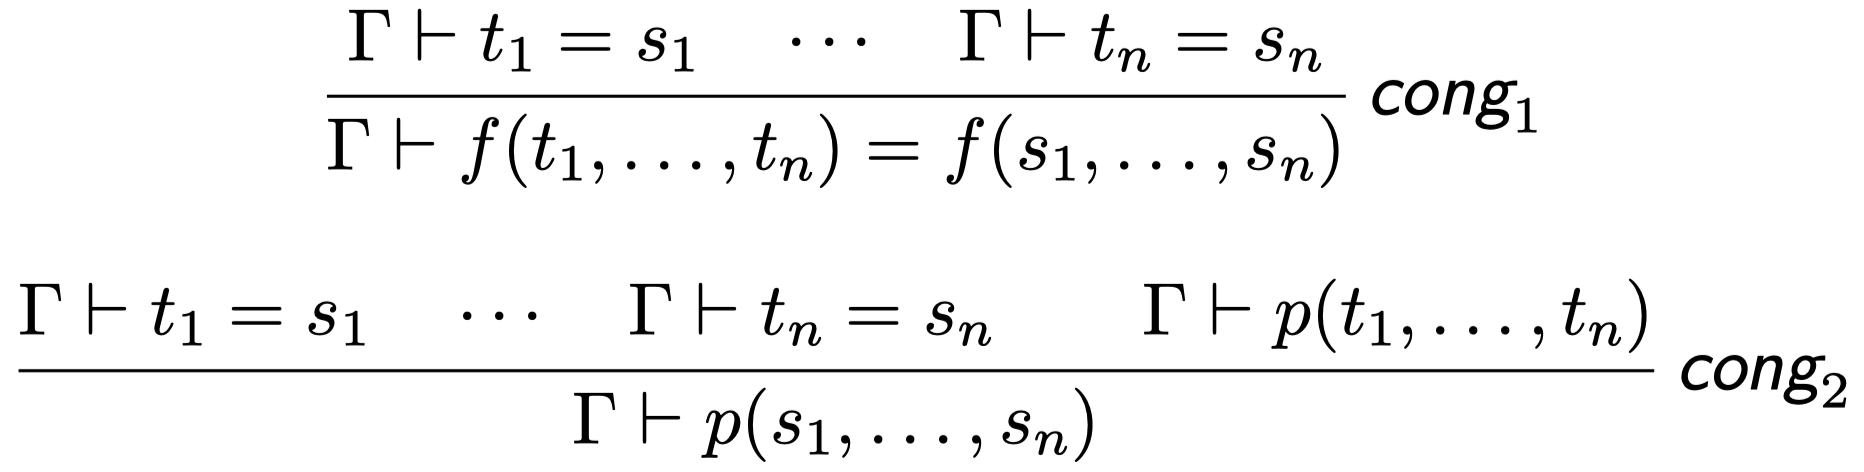
\includegraphics[width=11cm]{../images/FMFP_Fig2-5}
    \centering
\end{figure}

\subsection{Correctness}

\textbf{Correctness} is important! But what does correctness mean? What properties should hold?

\begin{itemize}
    \item \textit{Termination:} Important for many, but not all, programs.
    \item \textit{Functional behavior:} Function should return "correct" value.
\end{itemize}

\subsubsection{Termination}

If \(f\) is defined in terms of functions \(g_1,..., \, g_k \, (g_i \neq f)\), and each \(g_i\) terminates, then so does \(f\). The problem we encounter here is \textit{recursion,} i.e. when some \(g_i = f\).

A sufficient condition for termination is that arguments must be smaller along a well-founded order on function's domain:

\begin{itemize}
    \item An order \(>\) on a set \(S\) is \textbf{well-founded} iff. there is no infinite decreasing chain \(x_1 > x_2 > x_3 > ...\) for \(x_i \in S\).
\end{itemize}

We can construct new well-founded relations from existing ones:

Let \(R_1\) and \(R_2\) be binary relations on a set \(S\). The composition of \(R_1\) and \(R_2\) is defined as:

\[
    R_2 \circ R_1 \equiv \{(a, \, c) \in S \times S \, | \, \exists b \in S.a \, R_1 \, b \land b \, R_2 \, c\}
\]

Note: For binary relation \(R\), we write \(a \, R \, b\) for \((a, \, b) \in R\).

Let \(R \subseteq S \times S\). Define:

\begin{align*}
    R^1 &\equiv R \\
    R^{n + 1} &\equiv R \circ R^n, \text{ for } n \geq 1 \\
    R^+ &\equiv \bigcup_{n \geq 1} R^n
\end{align*}

So \(a \, R^+ \, b\) iff. \(a \, R^i \, b\) for some \(i \geq 1\).

\begin{cbox}
    \textbf{Lemma:} Let \(R \subseteq S \times S\). Let \(s_0, \, s_i \in S\) and \(i \geq 1\). Then \(s_0 \, R^i \, s_i\) iff. there are \(s_1,..., \, s_{i-1} \in S\) such that \(s_0 \, R \, s_1 \, R \, ... \, R \, s_{i - 1} \, R \, s_i\).
\end{cbox}

\begin{tbox}
    \textbf{Theorem:} If \(>\) is a well-founded order on set \(S\), then \(>^+\) is also well-founded on \(S\).
\end{tbox}

\begin{ebox}
    \textbf{Example:} Consider the following function:

    \begin{verbatim}
        fac 0 = 1
        fac n = n * fac (n - 1)
    \end{verbatim}

    \verb|fac n| has only \verb|fac (n - 1)| as a recursive call, and \(n > n -1\). Here, \(>\) is the standard ordering over the natural numbers. Therefore, the function terminates.
\end{ebox}

\subsubsection{Proofs}

Consider the following program:

\begin{verbatim}
    maxi :: Int -> Int -> Int
    maxi n m
        | n >= m    = n
        | otherwise = m
\end{verbatim}

Can we prove that \verb|maxi n m >= n|? We to a \textbf{reasoning by cases:}

We have \(n \geq m \lor \lnot (n \geq m)\). Now we show that \verb|maxi n m >= n| for both cases:

\begin{itemize}
    \item Case 1: \(n \geq m\), then \verb|max n m = n| and \(n \geq n\).
    \item Case 2: \(\lnot (n \geq m)\), then \verb|maxi n m = m|. But \(m > n\), so \verb|maxi n m >= n|.
\end{itemize}

But how do we prove a formula \(P\) (with free variable \(n\)), for all \(n \in \mathcal{N}\)? For example, how do we prove the following equality:

\[
    \forall n \in \mathcal{N} . 0 + 1 + 2 + ... + n = n \cdot (n + 1) / 2
\]

We can do a \textbf{proof by induction:}

\begin{itemize}
    \item Base case: Prove \(P[n \to 0]\)
    \item Step case: For an arbitrary \(m\) not free in \(P\), prove \(P[n \to m + 1]\) under the assumption \(P[n \to m]\).
\end{itemize}

\begin{ebox}
    \textbf{Example:} We have the following conjecture: \(\forall n \in \mathcal{N}.(\text{sumPowers } n) + 1 = \text{power2 } (n + 1)\) with the following code:

    \begin{verbatim}
        power2 :: Int -> Int
        power2 0 = 1
        power2 r = 2 * power2 (r - 1)

        sumPowers :: Int -> Int
        sumPowers 0 = 1
        sumPowers r = sumPowers (r - 1) + power2 r
    \end{verbatim}

    We want to proof: Let \(P \equiv (\text{sumPowers } n) + 1 = \text{power2 } (n + 1)\). We show \(\forall m \in \mathcal{N} . P\) by induction on \(n\).

    \paragraph{Base case:} Show \(P[n \to 0]\):
    \begin{align*}
        (\text{sumPowers } 0) + 1 &= 1 + 1 = 2 \\
        \text{power2 } (0 + 1) &= 2 \cdot \text{power2 } 0 = 2 \cdot 1 = 2
    \end{align*}

    \paragraph{Step case:} Assume \(P[n \to m]\) for an arbitrary \(m\) (not in \(P\)), i.e.
    \[
        (\text{sumPowers } m) + 1 = \text{power2 } (m + 1)  
    \]
    and prove \(P[n \to m + 1]\), i.e.
    \[
        (\text{sumPowers } (m + 1)) + 1 = \text{power2 } ((m + 1) + 1).  
    \]
    Proof:
    \begin{align*}
        (\text{sumPowers } (m + 1)) + 1 &= \text{sumPowers } ((m + 1) - 1) + \text{power2 } (m + 1) + 1 \quad (\text{def.}) \\
        &= \text{sumPowers } (m) + 1 + \text{power2 } (m + 1) \quad (\text{arithmetic}) \\
        &= \text{power2 } (m + 1) + \text{power2 } (m + 1) \quad (\text{ind- hypothesis}) \\
        &= 2 \cdot \text{power2 } (m + 1) \quad (\text{arithmetic}) \\
        &= \text{power2 } (m + 2) \quad (\text{def.})
    \end{align*}
    We have proven \((\text{sumPowers } n) + 1 = \text{power2 } (n + 1)\).
\end{ebox}

The general schema for \textbf{well-founded induction} is given as:

\begin{itemize}
    \item \textit{To prove:} \(\forall n \in \mathcal{N}.P\)
    \item \textit{Fix:} An arbitrary \(m\) not free in \(P\)
    \item \textit{Assume:} \(\forall l \in \mathcal{N} . l < m \to P[n \to l]\) (\textit{induction hypothesis})
    \item \textit{Prove:} \(P[n \to m]\)
\end{itemize}

\section{More on Haskell}

\subsection{List and Abstraction}

\subsubsection{List Type}

We introduce a new type constructor: \textbf{List types,} i.e. if \(T\) is a type, then \([T]\) is a type. The elements of \([T]\) are:

\begin{itemize}
    \item \textit{Empty list:} \verb|[] :: [T]|
    \item \textit{Non-empty list:} \verb|(x : xs) :: [T]|m if \verb|x :: T| and \verb|xs :: [T]|
\end{itemize}

\textit{Syntactic sugar:} We can write \verb|1 : (2 : (3 : []))| as \verb|[1, 2, 3]|.

\end{document}